\clearpage

\subsection{例題11 シューティングゲームの内容を改造する}

\subsubsection*{考え方}

シューティングゲーム(shoot.hsp)のスクリプトを改造してゲームの内容を変えてみましょう。
シューティングゲームのスクリプトは、「/home/ユーザー名/02/shoot.png」というファイルに保存されています。

まず、HSPスクリプトエディタを起動して、ファイル→「開く」メニューから「shoot.hsp」を読み込んでください。

\begin{figure}[H]
    \begin{center}
        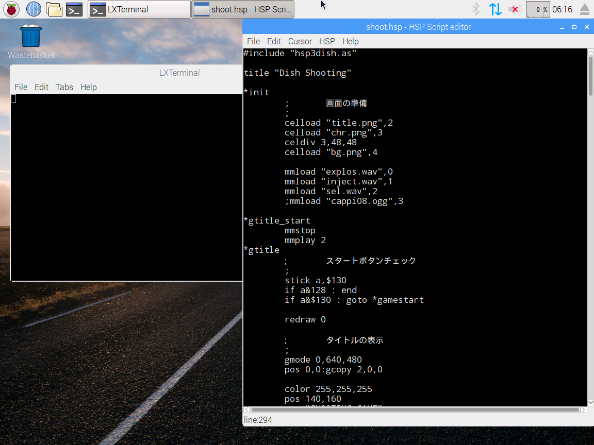
\includegraphics[keepaspectratio,width=6.853cm,height=5.135cm]{text02-img/text02-img043.png}
        \caption{shoot.hspを読み込んだところ}
    \end{center}
\end{figure}

でたらめに書き直してもエラーが出るだけです。
タイトルに表示されている文字、色、場所はパラメーターを変えられます。
命令にあたる部分は変えないようにしましょう。

\begin{itemize}
    \item プレイヤーのミサイル\ruby{連射}{れん|しゃ}を増やしてみる
\end{itemize}

\begin{description}
    \item (「lmax=4」が連射の数です)
    \item 敵の数を変えてみる
    \item (「einter=18」が出てくる確率「emax=16」が最大の数です)
    \item 敵の弾数を変えてみる
    \item (「msrint=2」の2を大きくすると増えます「amax=16」は最大の数です)
    \item ゲームの速度を変えてみる
    \item (「await 18」という部分の18を少ない数にしてみましょう)
\end{description}

\subsubsection*{例題11 答え}

ゲームを改造することで、\ruby{難}{むずか}しくなったり、簡単になったりします。
改造ができたらTAや周りの友達にも見せてあげましょう。

※プログラムをあまり改造しすぎると、動かなくなったり、パソコンの動きが遅くなってしまうことがあります。その時は、先生に聞くか、「/usr/local/share/ome/02/」フォルダ内の元のファイル(shoot.hsp)をもう一度コピーして使ってみてください。
